\documentclass[12pt, titlepage]{article}

\usepackage{fullpage}
\usepackage[round]{natbib}
\usepackage{multirow}
\usepackage{booktabs}
\usepackage{tabularx}
\usepackage{graphicx}
\usepackage{float}
\usepackage{hyperref}
\usepackage[shortlabels]{enumitem}
\usepackage{amsmath, mathtools}
\usepackage{amsfonts}
\usepackage{amssymb}
\usepackage{colortbl}
\usepackage{xr}
\usepackage{longtable}
\usepackage{xfrac}
\usepackage{siunitx}
\usepackage{caption}
\usepackage{pdflscape}
\usepackage{afterpage}
\usepackage{titlesec}
\usepackage{array}
\hypersetup{
    colorlinks,
    citecolor=blue,
    filecolor=black,
    linkcolor=red,
    urlcolor=blue
}
\usepackage{graphicx}
\graphicspath{ {./images/} }
\usepackage{caption}
\usepackage{enumitem}
\input{../../Comments}
%% Common Parts

\newcommand{\progname}{Chess Connect} % PUT YOUR PROGRAM NAME HERE
\newcommand{\authname}{Team \#4,
\\ Alexander Van Kralingen
\\ Arshdeep Aujla
\\ Jonathan Cels
\\ Joshua Chapman
\\ Rupinder Nagra} % AUTHOR NAMES without MacIDs 

\usepackage{hyperref}
    \hypersetup{colorlinks=true, linkcolor=blue, citecolor=blue, filecolor=blue,
                urlcolor=blue, unicode=false}
    \urlstyle{same}

\newcommand{\projectoverview}{

The Chess Connect project allows two users to play a game of chess on a physical board with the information being transmitted to an online web application over Bluetooth.
Currently, there is no way for players to seamlessly switch between playing on a physical board and playing online, but Chess Connect intends to change this by creating a central platform that will provide flexibility and remove barriers for new players looking to learn the game.

}

\newcounter{acnum}
\newcommand{\actheacnum}{AC\theacnum}
\newcommand{\acref}[1]{AC\ref{#1}}

\newcounter{ucnum}
\newcommand{\uctheucnum}{UC\theucnum}
\newcommand{\uref}[1]{UC\ref{#1}}

\newcounter{mnum}
\newcommand{\mthemnum}{M\themnum}
\newcommand{\mref}[1]{M\ref{#1}}

\begin{document}

\title{System Design for \progname} 
\author{\authname}
\date{\today}

\maketitle

\pagenumbering{roman}

\section{Revision History}

\begin{tabularx}{\textwidth}{p{3cm}p{2cm}X}
\toprule {\bf Date} & {\bf Version} & {\bf Notes}\\
\midrule
2023-01-11 & Arshdeep Aujla & Introduction, Purpose, User Interface, Other Considered Designs \\
2023-01-17 & Arshdeep Aujla & Added Design of Hardware \\
2023-01-18 & Joshua Chapman & Scope, Project Overview, System Variables, Timeline\\
2023-01-18 & Joshua Chapman & Hardware Design, Communication Protocols, Wiring Diagram\\
2023-01-18 & Rupinder Nagra & Interface\\
\bottomrule
\end{tabularx}

\newpage

\section{Reference Material}

This section records information for easy reference.

\subsection{Abbreviations and Acronyms}

\subsection{Abbreviations and Acronyms}

\renewcommand{\arraystretch}{1.2}
\begin{tabular}{l l} 
  \toprule		
  \textbf{symbol} & \textbf{description}\\
  \midrule 
  M & Module \\
  MG & Module Guide \\
  R & Requirement\\
  SC & Scientific Computing \\
  SRS & Software Requirements Specification\\
  \progname & Explanation of program name\\
  UC & Unlikely Change \\
  \bottomrule
\end{tabular}\\

\newpage

\tableofcontents

\newpage

\listoftables

\listoffigures

\newpage

\pagenumbering{arabic}

\section{Introduction}
This document outlines the system design portion of this project's design documentation. Design documentation 
is intended to separate the project into modular components to increase the project's understandability and reusability. \\
Other useful documents for this project are the following:
\begin{itemize}
  \item SRS
  \item HA
  \item VnV
\end{itemize}

\section{Purpose}
The purpose of this document is to outline a detailed system design. The system design includes system variables, user interfaces, a timeline for completion, and designs of many 
different components such as hardware, electrical components, and communication protocols. This document also includes references to an intensive list of the project's
mechanical and electrical components and a reflection in the appendix. \\
Other documents relating to design are the following:
\begin{itemize}
  \item Software Architecture Document
  \item Detailed Design Document
\end{itemize}
\section{Scope}
The Chess Connect system includes a physical chess board and associated software 
application to aid in the learning and sharing of in-person chess games. 
Mechanical design of the chess board and electrical systems are included in the 
scope. Design of the user interface and communication between the systems is also
included. 
Not included is the design of the chess AI being used as a learning tool. Exisiting
chess websites and platforms are also out of the scope of Chess Connect.

\begin{figure}[H]
  \begin{center}
    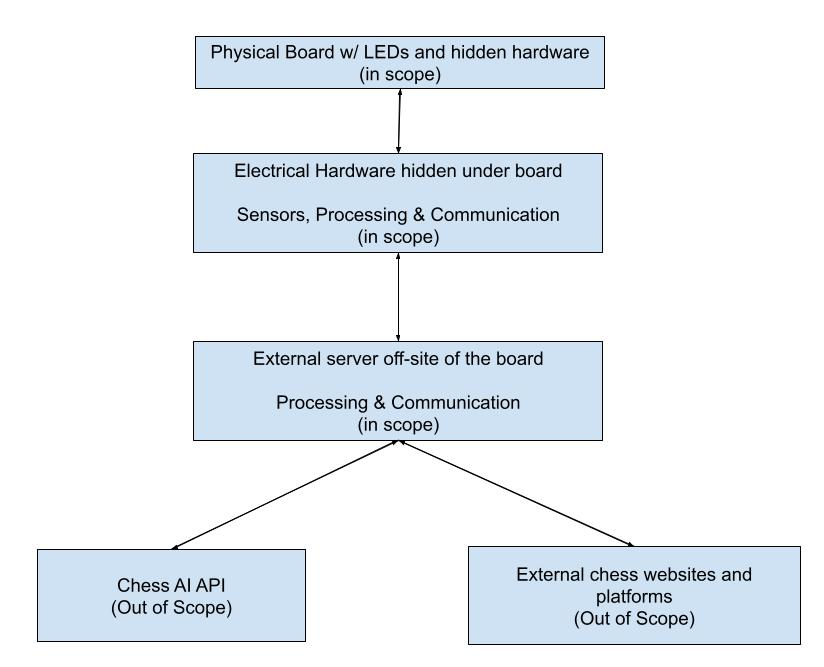
\includegraphics[scale=0.45]{scope.jpg}
    \caption{System Scope}
    \label{Fig_Scope} 
  \end{center}
\end{figure}
%Include a figure that show the System Context showing the boundary between
%your system and the environment around it.

\section{Project Overview}

\subsection{Normal Behaviour}{
The normal operation of the chess board involves configuring game mode and settings, reading the physical 
positions and identifiers (magnetic strength) of the pieces, lighting up corresponding LEDs and determining 
legal moves on the micro-controller. There will be three game modes: Normal Mode (no LED feedback), Engine 
Mode (best moves calculated by a chess engine and displayed by an LCD display) and Beginner Mode (legal moves
 displayed by LED when a piece is picked up). The micro-controller will also be simultaneously transmitting 
 data to the server via Bluetooth and receiving responses in the form of ``best'' moves from the server. The 
 server will be calculating these best moves in real time depending on the configuration of the pieces on the 
 board sent from the chess board, and sending it back over Bluetooth every time it is queriedwhile the game is
  in ``Engine Mode''. The server will also be communicating all of this information to a web application where 
  users can tune in and watch the pieces and seegame stats in real time.
}

\subsection{Undesired Event Handling}
When an unexpected event occurs, chess connect will always return to the most 
appropriate safe state. When an action during a game, the on-board LCD screen 
displays the error and provides instructions to correct the mistake and proceed 
normally. When an error occurs in the communication between sub-systems, all 
activememory is stored and a default error screen appears on the LCD screen to 
inform the players.
%\wss{How you will approach undesired events}

\subsection{Component Diagram}
\begin{figure}[H]
  \begin{center}
    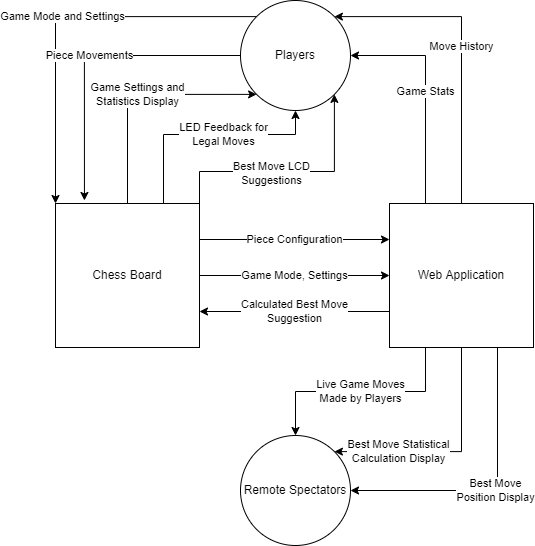
\includegraphics[scale=0.65]{chess-connect-system-context.png}
    \caption{Overall System Context}
    \label{Fig_SystemContext} 
  \end{center}
\end{figure}


\subsection{Connection Between Requirements and Design} \label{SecConnection}

Requirements GA1, GA2, GA3, GA4, GI1, GI2, GI3, NB2, NB3, EB2, EB3, EB4, BB3, BB4, BB5 describe a variety of 
buttons to support game flow and modes. Too many physical buttons were required so an LCD screen was placed on 
the side of the board to accomodate the large number of functions. 
\\ \\
Requirements GI5, GI6, ND1, NA1, ED1, ED2, EA1, BD1 dictated decisions for specific information to be 
communicated from the board to the Web Application. Serial Communication was chosen to display a custom 
string to communicate the necessary game state, errors and best moves between the board and the application. 
\\ \\
Requirements NB1, EB1, BB1 describe the memory performance required of the hardware to store game data of 
entire games. Design satisfies this requirement with the addition of two processors to share the memory load
and processing load.
\\ \\
Requirement BB2 outlined the implementation of LEDs requiring fast response times. Due to communication 
protocols, screens and sensors are already consuming processor time, a second processor was added with faster 
processing speed to handle the LEDs and sensors exclusively.
%wss{The intention of this section is to document decisions that are made
%  ``between'' the requirements and the design.  To satisfy some requirements,
 % design decisions need to be made.  Rather than make these decisions implicit,
  %they are explicitly recorded here.  For instance, if a program has security
  %requirements, a specific design decision may be made to satisfy those
  %requirements with a password.}

\section{System Variables}
%\wss{Include this section for Mechatronics projects}
\subsection{Monitored Variables}
\begin{table}[H]
  \centering
      \setlength{\leftmargini}{0.4cm}
      \begin{tabular}{| >{\centering\arraybackslash}m{2.5cm} | 
        >{\centering\arraybackslash}m{2cm} | 
        >{\centering\arraybackslash}m{9cm} |}
      \hline
      \rowcolor[gray]{0.9}
      Variable & Units & Description\\
      \hline
      s\_a\{1-8\} & Volts & States of tiles a1 - a8 on the board. They are analog signals 
      converted to digital and the state of the tile is determined. The possible states of 
      each tile is empty, black/white pawn, black/white rook, black/white knight, 
      black/white bishop, black/white queen, black/white king. \\
      \hline
      s\_b\{1-8\} & Volts & States of tiles b1 - b8 on the board. " " \\
      \hline
      s\_c\{1-8\} & Volts & States of tiles c1 - c8 on the board. " " \\
      \hline
      s\_d\{1-8\} & Volts & States of tiles d1 - d8 on the board. " " \\
      \hline
      s\_e\{1-8\} & Volts & States of tiles e1 - e8 on the board. " " \\
      \hline
      s\_f\{1-8\} & Volts & States of tiles f1 - f8 on the board. " " \\
      \hline
      s\_g\{1-8\} & Volts & States of tiles g1 - g8 on the board. " " \\
      \hline
      lcd\_x\_pos & Volts & Positive X coordinate of the resistive touch screen.\\
      \hline
      lcd\_x\_neg & Volts & Negative X coordinate of the resistive touch screen.\\
      \hline
      lcd\_y\_pos & Volts & Positive Y coordinate of the resistive touch screen.\\
      \hline
      lcd\_y\_neg & Volts & Negative Y coordinate of the resistive touch screen.\\
      \hline
      bluetooth\_rx & Volts & Serial communication receive channel via bluetooth to the web application.
      Best moves from the chess engine are sent to the chess board via this channel. \\
      \hline 
      \end{tabular}
  \label{Table}
  \end{table}

\subsection{Controlled Variables}
\begin{table}[H]
  \centering
      \setlength{\leftmargini}{0.4cm}
      \begin{tabular}{| >{\centering\arraybackslash}m{3cm} | 
        >{\centering\arraybackslash}m{2cm} | 
        >{\centering\arraybackslash}m{9cm} |}
      \hline
      \rowcolor[gray]{0.9}
      Variable & Units & Description\\
      \hline 
      hall\_power\{1-8\} & Volts & Eight sources of power to the eight columns of sensors under the board. 
      The power will be pulse width modulated to multiplex the signals of the hall sensors.\\
      \hline 
      LED\_row\_pos\{1-9\} & Volts & Nine power supplies are delivered to the nine rows of LEDs. When a 
      corresponding ground is supplied to a column, an individual LED can be lit.\\
      \hline
      LED\_col\_gnd\{1-9\} & Volts & Nine ground supplies are delivered to the nine columns of LEDs. When a 
      corresponding power is supplied to a row, an individual LED can be lit.\\
      \hline 
      LCD\_Display\{0-7\} & Volts & Eight bits of information are sent to the LCD screen to display a variety
      of images. \\
      \hline 
      bluetooth\_tx & Volts & Serial communication transmit channel via bluetooth to the web application. 
      The current game state and errors are sent via this channel. \\
      \hline
      \end{tabular}
  \label{Table}
  \end{table}

\subsection{Constants Variables}
\begin{table}[H]
  \centering
      \setlength{\leftmargini}{0.4cm}
      \begin{tabular}{| >{\centering\arraybackslash}m{5cm} | 
        >{\centering\arraybackslash}m{2cm} | 
        >{\centering\arraybackslash}m{5cm} |}
      \hline
      \rowcolor[gray]{0.9}
      Constant & Unit & Value\\
      \hline
      Chess board width & inches & 12\\
     \hline
     Chess board length & inches & 12\\
     \hline
     Chess board tile width & inches & 1.5\\
     \hline 
     Chess board tile length & inches & 1.5\\ 
     \hline 
     Supply Power to Board & Volts & 110 VAC\\
     \hline
      \end{tabular}
  \label{Table}
  \end{table}

\section{User Interfaces}

\subsection{Hardware Interface}
The user will interact with two main components of the hardware.
\begin{itemize}
  \item Magnetic chess pieces
  \item Physical chess board containing sensors
\end{itemize}
They will interact with the chess pieces and chess board as they would in a normal chess game. The chess board reflects a standard chess board, with 
LEDs in the center of each square. They would move the chess pieces on the board and remove them in according to the rules of chess. If the device
is set to beginner mode, the LEDs will light up in according to which available moves are available for that chess piece. They would interact with the LEDs
by using them as a guide for potential moves to make.

\subsection{Software Interface}
The users will interact with the software component of this device through a web application. They would need a device with an internet connection and and internet browser
to view the application. The user will interact with this interface by visual viewing the chess board status in real time including a visualization of the chess piece locations.
They will also be able to turn on and off beginner mode in this interface through clicking an interactive button in the web application. 

\section{Design of Hardware}
To build the custom chess board for Chess Connect we designed a modified chess 
board to fulfill the requirements of the system. The chess board has visible 
LEDs from below the board that can be seen in the figure below. 
\begin{figure}[H]
  \begin{center}
    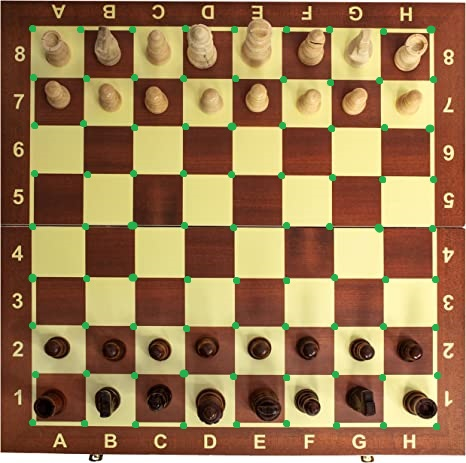
\includegraphics[scale=0.75]{chess_board.jpg}
    \caption{Hardware Design}
    \label{Fig_Hardware_Design} 
  \end{center}
\end{figure}
The chess board will be hollow and contain enough space to contain the 
electronics. An AC power cable will protrude from the side of the board to 
connect to an outlet nearby. 




\subsection{Components Acquired}
Please refer to Appendix B for a detailed list of acquired mechanical components.

\section{Design of Electrical Components}
\subsection{Components Acquired}
Please refer to Appendix C for a detailed list of acquired electrical components.

\subsection{Wiring Diagram}
\begin{figure}[H]
  \begin{center}
    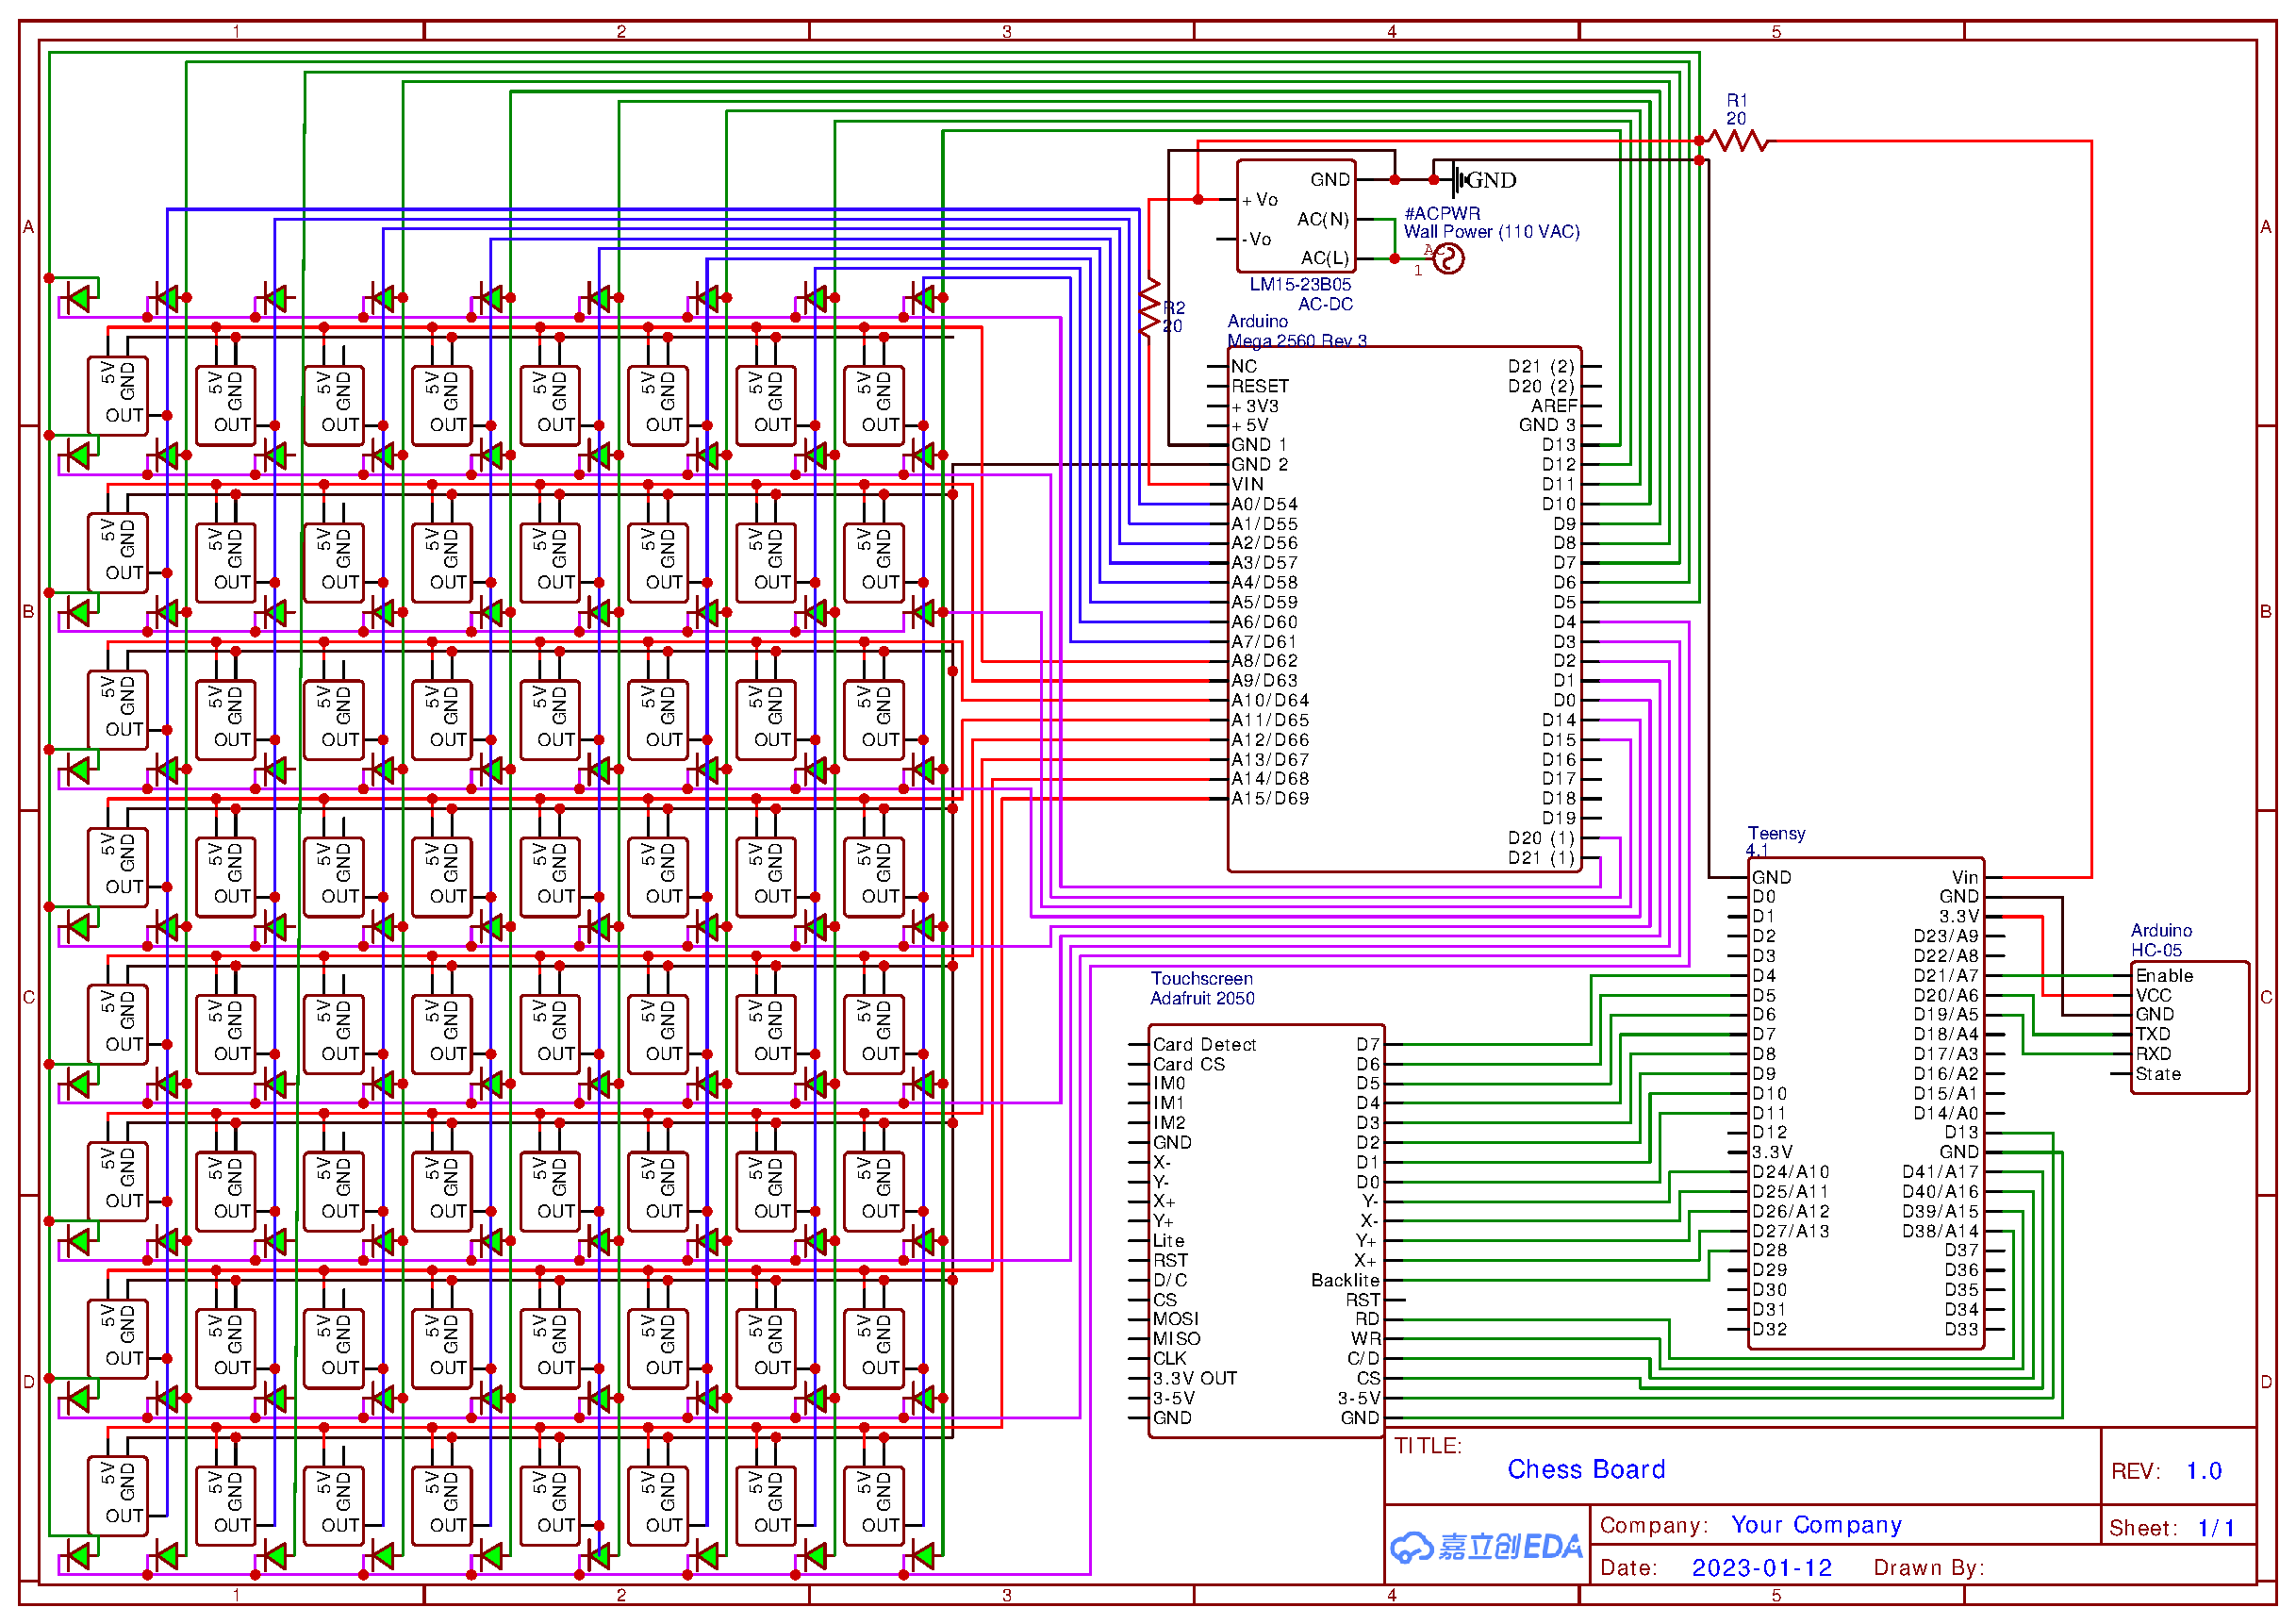
\includegraphics[scale=0.45]{wiring_diagram.pdf}
    \caption{Electrical Wiring Diagram}
    \label{Fig_Wiring_Dgm} 
  \end{center}
\end{figure}

\subsection{LED and Piece Interaction}
Each square on the chessboard will contain a Hall sensor and a green LED. The LEDs are to indicate where a piece can possibly go, depending on which mode the user is in. For example, 
if the user is in a beginner’s mode and picks up the White King, then the LEDs surrounding all the squares where the King is picked up from will light up telling the user that the 
King can be placed on any of those squares. The logic for which LEDs light up depend on a few things:
\begin{itemize}
  \item The type of piece. Different LEDs would light up for King, Queen etc.
  \item If any of the user’s own color piece is placed on a square, that LED would not light up as you cannot place two pieces on the same square. However, if an opponent’s piece is 
  placed on a square, that LED may light up provided it is a valid move depending on the type of piece the user is making the move with.
  \item Any square further away from a square where user’s own piece is present, will not light up as the pieces cannot jump a piece unless it is a Knight.
\end{itemize}
  Let us see the working of the LEDs considering the example on a 5x5 grid as shown in the figure below. ‘1-5’ are the rows and ‘A-E’ are the columns. ‘a-e’ are the twenty-five different LEDs corresponding to 
  each square. The green background squares will indicate the LED to be ON for that square in the grid.

  \begin{figure}[h]
    \centering
    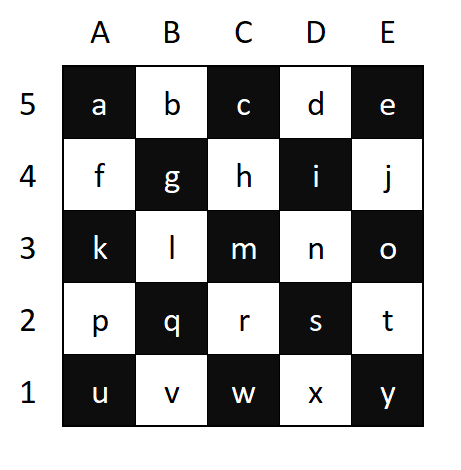
\includegraphics[width=0.5\textwidth]{line2}
    \caption{5x5 Grid}
  \end{figure}

  \begin{itemize}
    \item Case 1: King present in the middle of a 5x5 grid chessboard. The King can move only one square in any direction – up, down, to the sides, and diagonally.

    \begin{minipage}{\linewidth}
      \centering
      
\includegraphics[width=0.5\textwidth]{king}
      \captionof{figure}{Potential moves for the King}
  \end{minipage}

  The LEDs g,h,i,l,n,q,r,s will light up for the potential moves provided those squares are empty or an opponent’s piece is placed on those squares.

    \item Case 2: Queen present in the middle of a 5x5 grid chessboard. The Queen can move multiple squares in any one direction - forward, backward, sideways and 
    diagonally as far as possible as long as she does not move through any of her own pieces.

    \begin{minipage}{\linewidth}
      \centering
      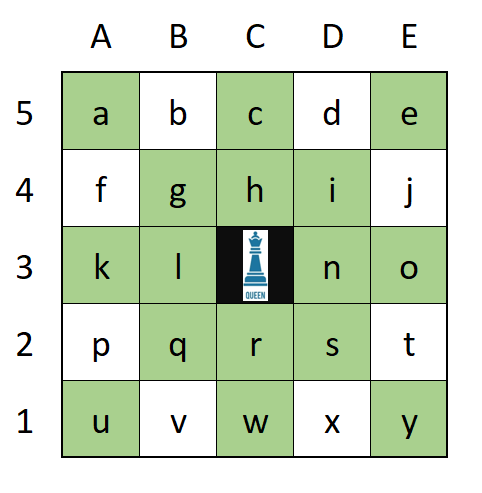
\includegraphics[width=0.5\textwidth]{queen}
      \captionof{figure}{Potential moves for the Queen}
  \end{minipage}

  The LEDs a,c,e,g,h,i,k,l,n,o,q,r,s,u,w,y will light up for the potential moves provided those squares are empty or an opponent’s piece is placed on those squares.

    \item Case 3: Bishop present in the middle of a 5x5 grid chessboard. The Bishop can move multiple squares but only diagonally. Each bishop starts on one color (light or dark) 
    and must always stay on that color. 

    \begin{minipage}{\linewidth}
      \centering
      
\includegraphics[width=0.5\textwidth]{bishop}
      \captionof{figure}{Potential moves for the Bishop}
  \end{minipage}

  The LEDs a,e,g,i,q,s,u,y will light up for the potential moves provided those squares are empty or an opponent’s piece is placed on those squares.

    \item Case 4: Knight present in the middle of a 5x5 grid chessboard. The Knight can move two squares in one direction, and then one more move at a 90-degree angle in either 
    direction, just like the shape of an “L”. 

    \begin{minipage}{\linewidth}
      \centering
      
\includegraphics[width=0.5\textwidth]{knight}
      \captionof{figure}{Potential moves for the Knight}
  \end{minipage}

  The LEDs b,d,f,j,p,t,v,x will light up for the potential moves provided those squares are empty or an opponent’s piece is placed on those squares. Knight is the only chess 
  piece that can skip over a piece and be placed even if it is immediately surrounded by a user’s own piece. For example, if there is user’s own pieces present at the 
  squares B2, B3 and B4, the user can still place the Knight at A2, A4, B1 or B6 by skipping over the other pieces.

    \item Case 5: Rook present in the middle of a 5x5 grid chessboard. The Rook can move multiple squares but only forward, backward or to the sides. 
  
    \begin{minipage}{\linewidth}
      \centering
      
\includegraphics[width=0.5\textwidth]{rook}
      \captionof{figure}{Potential moves for the Rook}
  \end{minipage}

  The LEDs c,h,k,l,n,o,r,w will light up for the potential moves provided those squares are empty or an opponent’s piece is placed on those squares.

    \item Case 6: Pawn present in the middle of a 5x5 grid chessboard. Pawns are unusual because they move and capture in different ways: they move forward but capture 
    diagonally. Pawns can only move forward one square at a time, except for their very first move where they can move forward two squares.

    \begin{minipage}{\linewidth}
      \centering
      
\includegraphics[width=0.5\textwidth]{pawn}
      \captionof{figure}{Potential moves for the Pawn}
  \end{minipage}

  The LEDs c,g,h,i will light up for the potential moves provided those squares are empty or an opponent’s piece is placed on those squares. For pawn, the LED ‘c’ only 
  lights up if it is the first time a pawn is making a move. After a pawn has been moved once, it can never move two squares at once. Also, a pawn can move diagonally, 
  only if there is an opponent’s piece is present on those squares. Otherwise, it can only move in the forward direction. For example, the LED ‘g’ or ‘i’ will only light 
  up if there is an opponent’s piece present on them. 

  \end{itemize}
  


\subsection*{Truth Table for LEDs}

Based on the assumptions above, the Truth Table for the LEDs 'a-y' would as shown in the figure below. 
The digit '0' means LED is OFF and '1' means LED is ON.

\begin{figure}[h]
  \centering
  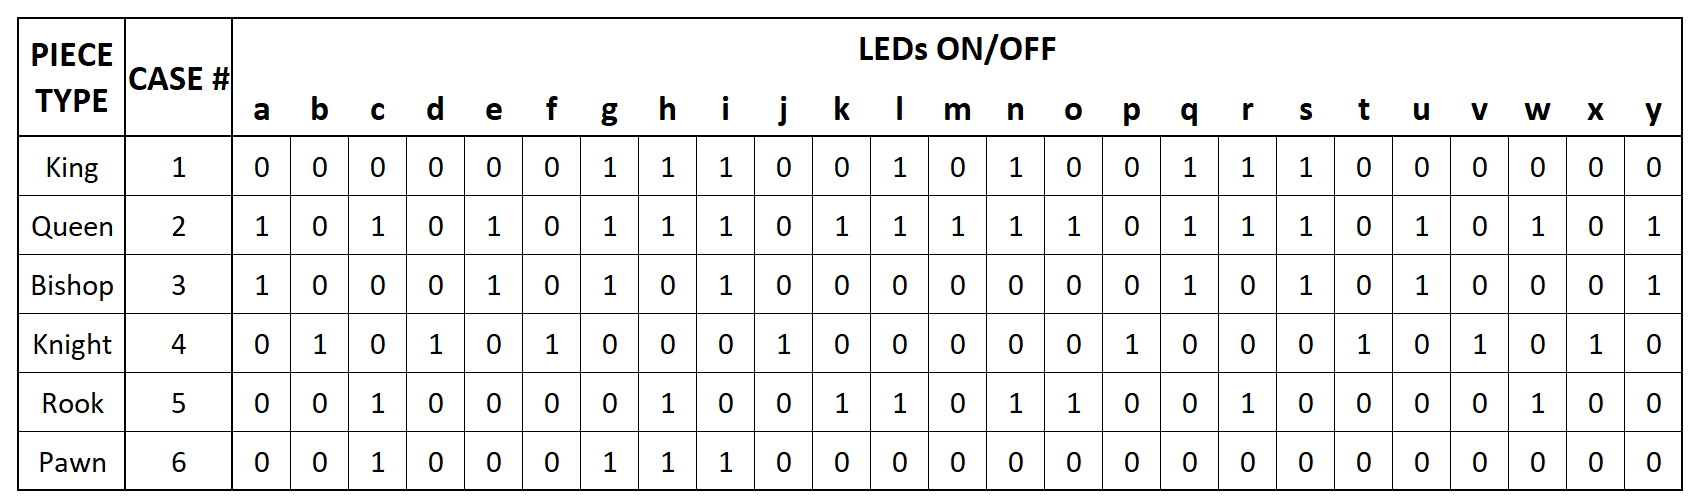
\includegraphics[width=1\textwidth]{truth_table}
  \caption{Truth Table}
\end{figure}
%\wss{Most relevant for mechatronics projects}
%\wss{Show what will be acquired}
%\wss{Show what will be built, with detail on fabrication and materials}
%wss{Include appendices as appropriate, possibly with sketches, drawings,
%circuit diagrams, etc}

\section{Design of Communication Protocols}

\subsection{Arduino Mega to Teensy}
The two processors communicate to share game state, game mode and move information for smooth 
performance. Arduino Mega collects data and forms the current game state from the sensors given. 
Once the current game state is formed it is sent via serial communication to the Teensy 
processor. The string is in the form of FEN@Game Mode@Resign. 
\subsection{Web Application to Teensy}
The processor and the web application communicate to share current game state, game mode and 
best moves from the engine. The Teensy sends a string in from of FEN@Game Mode to the web application
to perform best move calculations. Once the web application finds the best moves, it will send a
string in the form of bestMove1@bestMove2@bestMove3 back to the Teensy.
%\wss{If appropriate}

\section{Timeline}
\begin{table}[H]
  \centering
      \setlength{\leftmargini}{0.4cm}
      \begin{tabular}{| >{\centering\arraybackslash}m{10cm} | 
        >{\centering\arraybackslash}m{2cm} | 
        >{\centering\arraybackslash}m{1.5cm} |}
      \hline
      \rowcolor[gray]{0.9}
      Task & Member & Date\\
      \hline 
      Learning the library of the LCD screen & Josh & Jan 23\\
      \hline
      Learning the library of the bluetooth module for web app communication & Jonathan & Jan 23\\
      \hline 
      Installing the hall sensors and LEDs to the bottom of the chess board & Arshdeep & Jan 23\\
      \hline
      Complete design and implementation of web application & Rupinder & Jan 30\\
      \hline 
      Solder sensors and LEDs to the appropriate Arduino & Arsheep & Jan 30\\
      \hline 
      Configure power supply for arduinos and confirm safety of the system from wall power & Josh & Jan 30\\
      \hline
      Implementing a chess library into the arduino Mega & Alex & Jan 30\\
      \hline 
      Implement communication protocols for bluetooth and serial communication onto the processors & Jonathan
      & Jan 30\\
      \hline 
      Complete communication protocol packet from web app to arduino & Rupinder & Feb 7\\
      \hline 
      Run tests with the completed piece tracking code with completed board & Alex & Feb 7\\
      \hline 
      Revision 0 Demonstration. Completed by this time will be piece recognition, LED response, communication 
      between processors, bluetooth communication, web application and LCD screen design
      & Josh, Arsheep, Alex, Rupinder, Jonathan & Feb 13\\
      \hline
      
      \end{tabular}
  \label{Table}
  \end{table}
%\wss{Schedule of tasks and who is responsible}

% \bibliographystyle {plainnat}
% \bibliography{../../../refs/References}

\newpage{}

\appendix

\section{Interface}
An online chess game typically has a user interface that includes a chess 
board display, where the player can see the current state of the game and make
 moves. Our web application will only serve as an additional display for the 
 moves being played on the physical board, simply mirroring the moves with 
 minimal latency over Bluetooth. The different modes on the physical board 
 will also be compatible with the moves displayed on the web application. A 
 web application interface aims to be more intuitive for players that are 
 accustomed to online chess and might also allow for a more immersive viewing
 experience for spectators.

%\wss{Include additional information related to the appearance of, and
%interaction with, the user interface}

\section{Mechanical Hardware}
\begin{itemize}
  \item 20" Chess Board
  \item Self Contained Box to hide hardware
\end{itemize}

\section{Electrical Components}
\begin{itemize}
  \item Arduino Mega 2560
  \item Teensy 4.1 
  \item 3.5" Touchscreen Display
  \item HC-05 Bluetooth Module
  \item AC-DC converter for 
  \item 81 green LEDs
  \item 81 1000ohm resistors
  \item 64 HALL sensors
  \item 64 1mF capacitors
  \item 30 ft, 20 AWG wire
\end{itemize}

\section{Reflection}

\subsection*{Project Limitations}

\subsection*{Other Considered Designs}
One problem that we had to overcome in our design is that there are not enough input and output pins in one microcontroller for all of the components.
One solution we considered was having multiple microcontrollers for this project to ensure there is one input pin for each input sensor and one output pin for each output.
This design would be beneficial in the way of simplicity of code. The tradeoff would be the complexity in coordinating the communication between multiple microcontrollers and the 
web application. A second option to solve this problem is to use multiplexing to reduce the number of input and output pins needed for a large number of components. 
This option requires more complex code, but only requires one microcontroller device. We chose to implement the multiplexing option because it only used one device which saves money,
as well as eliminates the need to coordinate between multiple microcontrollers. 

The information in this section will be used to evaluate the team members on the
graduate attribute of Problem Analysis and Design.  Please answer the following questions:

\begin{enumerate}
  \item What are the limitations of your solution?  Put another way, given
  unlimited resources, what could you do to make the project better? (LO\_ProbSolutions)
  \item Give a brief overview of other design solutions you considered.  What
  are the benefits and tradeoffs of those other designs compared with the chosen
  design?  From all the potential options, why did you select documented design?
  (LO\_Explores)
\end{enumerate}

\end{document}